\section{Aufbau}
\label{sec:Aufbau}
\begin{figure}
    \centering
    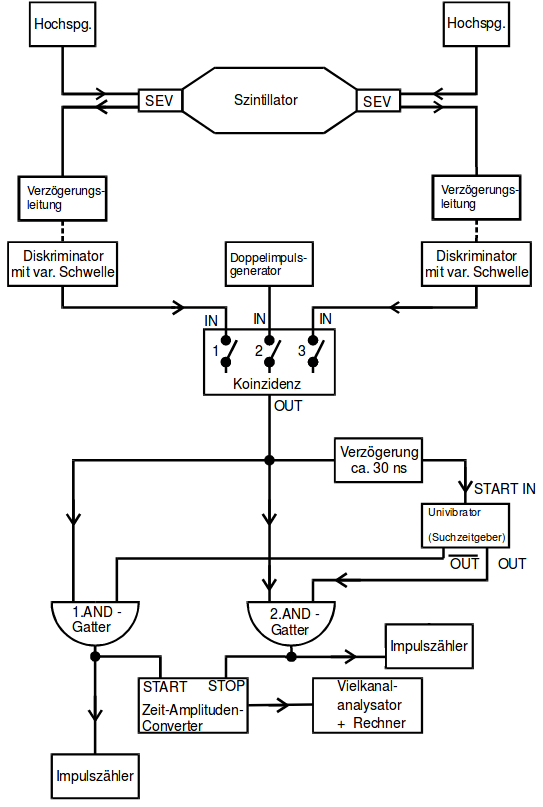
\includegraphics[width=0.9\textwidth]{content/images/AufbauV01.png}
    \caption{Die Messschaltung zur Aufnahme von Individuallebensdauern kosmischer Myonen.}
    \label{fig:Aufbau}
    \end{figure}
%Bild muss noch angepasst werden(zweite verzögerungsleitung, zweiter impulszähler)
%Der Aufbau besteht aus zwei Teilen. Der erste Teil filtert möglichst alle Impulse heraus, die aufgrund von. Im Anschluss folgt eine Schaltung, welche die individuellen Zerfallszeiten misst und sie in eine für den Computer verwertbare Form umformt.
%gehört die funktion vom szintillator hierrein
 Die in der Atmosphäre entstandenen Myonen gelangen zunächst in einen Szintillator. In diesem werden die zunächst noch relativistischen Myonen abgebremst, wobei sie ihre kinetische Energie an die umliegenden Moleküle abgeben. Diese werden daraufhin in energetisch höhere Niveaus gehoben und kehren daraufhin unter Aussendung eines Photons wieder in ihren Grundzustand zurück. Die Photonen liegen energetisch am oberen Rand des sichtbaren Spektrums. Um eine hohe zeitliche Genauigkeit zu erhalten, wird ein organischer Szintillator gewählt. Im Anschluss werden die Photonen mithilfe zweier Photomultiplier in elektrische Impulse umgewandelt und verstärkt.
  %Anschließend werden die Lichtquanten in zwei an beiden Seiten des Szintillators befestigten Photomultipliern in elektrische Signale umgewandelt und zur Verwertbarkeit um ca. um den Faktor $10^6$ verstärkt.
   Danach passieren die Impulse auf beiden Seiten eine Verzögerungsleitung und einen Diskriminator. In Letzteren werden die Signale einerseits von Störimpulsen niederer Spannung gefiltert und andererseits in eine einheitliche Form gebracht, welche von der nachfolgenden Koinzidenzapperatur benötigt wird.
    %Die zweite Stufe der Filterung von Störquellen bildet eine Koinzidenzapperatur.
     Diese gibt ein Signal aus, falls an beiden Eingängen Impulse im Abstand weniger Nanosekunden auftreten. Die Impulse des störenden Untergundes treten jedoch hauptsächlich aufgrund thermischer Elektronenemissionen im Anfangsbereich der Photomultiplier auf, weswegen es nur sehr unwahrscheinlich ist, dass 2 Impulse im benötigten Abstand auftreten. Die Photonen bewegen sich hingegen schnell genug, sodass die durch Myonen hervorgerufenen Impulse die Koinzidenzapperatur passieren können.
    %unterer teil der schaltung
    Mit dem zweiten Teil der Schaltung lässt sich die Lebensdauer der Myonen bestimmen. Hierzu werden Myonen geringerer Energie verwendet, welche bereits in der Atmosphäre ausreichend abgebremst worden sind und im Szintillator nun zum Stillstand kommen.
    % Da die vorherige Zeitdilatation nun aufhört zu wirken, kommt es zum Zerfall der Myonen.
    % sollte das mit den myonen vll doch eher in die theorie ?
    Da Myonen im Ruhesystem nur eine geringe Lebensdauer besitzen, kommt es zum Zerfall nach Formel $\eqref{eq:zerfall}$. Die entstehenden Produkte besitzen eine hohe kinetische Energie und werden ihrerseits im Szintillator abgebremst, wodurch ein zweiter Impuls ausgesendet wird. Die Zeitdifferenz beider Impulse liefert die individuelle Lebensdauer des Myons. Die Messschaltung nach Abb.$ \ref{fig:Aufbau}$ funktioniert folgendermaßen:
    Der erste Impuls läuft zu beiden AND-Gattern. Da das 1. AND-Gatter über den $\overline{\text{OUT}}$  und das 2. AND-Gatter über den OUT-Zugang eines Univibrators verbunden ist, wird der Impuls nur am 1. AND-Gatter durchgelassen. Er gelangt anschließend in den angeschlossenen Startimpulszähler und in den TAC, wo er die Zeitmessung startet. Mit ca. $\SI{30}{\nano\second}$ Verzögerung gelangt der Impuls auch in den Univibrator. Dieser klappt nun für eine eingestellte Zeit $T_\text{S}$ um. Gelangt in dieser Zeit ein zweiter Impuls in die Schaltung, wird dieser durch das 2. AND-Gatter in den TAC und einen zweiten Impulszähler für die Stops weitergeleitet. Der TAC stoppt daraufhin die Messung und gibt einen proportional zur Zeit angestiegenen Strom an einen angeschlossenen Vielkanalanalysator mit 512 Kanälen weiter. In diesem werden die Impulse nach ihrer Höhe in einzelne Kanäle einsortiert und in jedem einzelnen wird die eintreffenden Impulse gezählt. Die Messdaten können mit einem angeschlossenen Computer ausgelesen werden. Gelangt in der Zeit $T_\text{S}$ kein weiterer Impuls in die Schaltung, klappt der Univibrator wieder zurück und der nächste Impuls wird als neues Startsignal gewertet. Kommt es in der Zeit $T_\text{S}$ zur Abbremsung von zwei verschiedenen Myonen so werden diese als ein Zerfall gewertet. Dieser Untergrund lässt sich nicht herausfiltern und muss nachträglich bestimmt werden.